The purpose of this work is to study a short-time Fourier transform for its viability as a pitch detector. The FFT for transforming a waveform into the frequency-domain has been introduced and this chapter will focus on the properties of sound, introduce some musical terminology and how the FFT can be used to detecting pitches from a time-domain signal

\subsection{Basics of sound}
Sound physically is propagation through a medium, a vibration which some things can produce and some things can pick up. The word sound can be used to describe both the propagation itself, but also the phenomenom we feel when our ears react to the propagation. Speakers, strings of a guitar and vocal chords (together with the lungs) are some of the things that can produce sound and microphones and membranes in ears are things that can pick up sound. The propagation will have a certain strength at some point in the medium it travels through, which can be measured. This allows us to model the pressure propagation, or the sound as a function of time. At time $t$ the pressure at some point can be denoted as $f(t)$. This function over time can also be called a signal.

% source: https://api.pageplace.de/preview/DT0400.9781292055152_A24617782/preview-9781292055152_A24617782.pdf The Science of Sound - Rossing, Moore, Wheeler

One of the simplest ways to generate a sound is connecting a speaker to a device that generates an analog current in the shape of a wave. The current moves an electromagnet which moves a membrane at the same frequency as the generator. This membrane displaces air at some rate which ears pick up as sound. A 440Hz wave, a signal that oscillates 440 times per second that is, will produce a sound wave of 440Hz \todo{this most likely needs a source}. An ear picks up this signal as what we call an A4 note. Ironically, the purity of the signal makes it sound harsh and it is noise in the signal that gives warmth and beauty to the note. This can be observed in figure \ref{fig:pianoWave} where the signal (sound made by an electric piano) largely matches a pure A4 (440Hz sinusoid) but not quite.

%https://eprints.hud.ac.uk/id/eprint/17816/1/Final_Thesis_-_November_2012.pdf

\begin{figure}[ht]
    \centering
    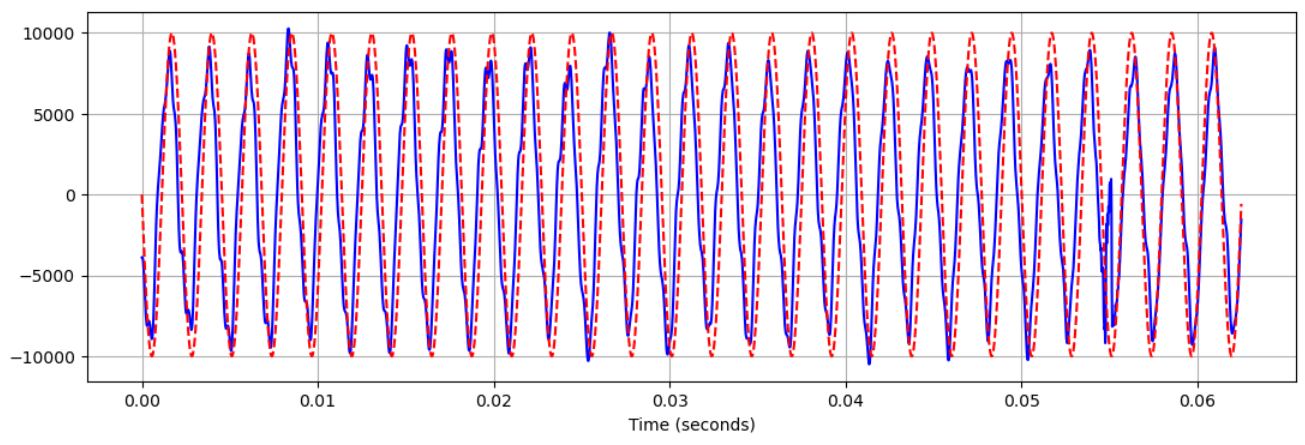
\includegraphics[width=\textwidth]{./images/piano_wave.png}
    \caption{A slice of the recording of a A4 note played on a Yamaha electric piano (blue solid). The signal contains a lot of irregularity but also clear regularity which becomes more evident when layering a pure A4 note on top (red dashed).\label{fig:pianoWave}}
\end{figure}

The characteristics of the sound being played becomes even more evident when it's converted to the frequency-domain through the FFT as shown in figure \ref{fig:pianoFreq}. It reveals that, not only is the sound definitely a A4 note due to the overwhelming amount of the 440Hz signal present in the sound, but also what other frequencies contribute to the sound of that piano.

\begin{figure}[ht]
    \centering
    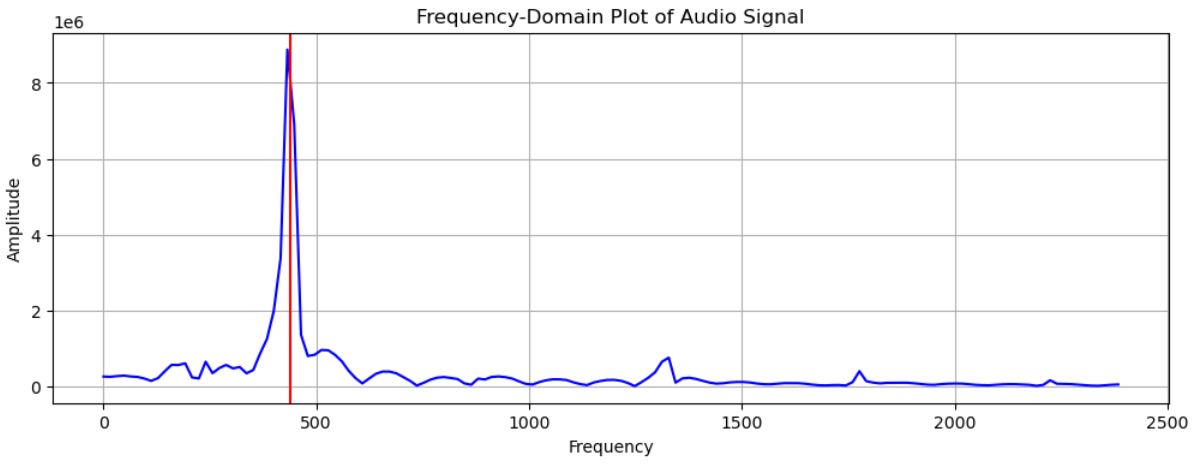
\includegraphics[width=\textwidth]{./images/piano_freq.png}
    \caption{The frequency-domain clearly reveals without any guesswork that the signal is a 440Hz signal with some sort of noise/disturbance. The red vertical line is placed at $x=440$ to show that the peak is the expected 440Hz frequency component.\label{fig:pianoFreq}}
\end{figure}

\subsubsection{Semitones, notes, frequency and pitch}
Semitone is typically defined as the smallest interval in western music and is 1/12th of an octave. Semitone is sometimes also used to talk about, not the interval, but the notes that bound the interval. This non-interval semitone is sometimes also called a pitch.   
An octave is the difference between some frequency $f_1$ and $f_2 = 2*f_1$, in other words going up an octave doubles the frequency. For example, the pitches F2 and F\#2 bound a semitone interval. In western music, tuning typically starts from A4, which is defined in this system to have a frequency of 440Hz, and every other note is derived from there. A3 (an octave lower) will be 220Hz and A5 will be 880Hz. The frequency for the other pitches can be approximated with equal temperament tuning, meaning that all semitones equally spaced within octaves. This means that the frequency of any one pitch is exactly $2^{1/12}$ times the frequency of the previous one. 

\subsection{Pitch detection}
There is no strict definition for pitch detection as pitch itself isn't very well defined . From a computational perspective, a possible definition is that pitch detection is the identification of the fundamental frequency and which is the corresponding semitone/pitch (because the note names are more valuable to musicians than the pure frequencies). The fundamental frequency is typically the lowest frequency of a signal, but in some cases we can hear a fundamental frequency that isn't actually a part of the signal, a phenomenon appropriately called the missing fundamental. \todo{source: Gotsopoulos}
% Why is it hard?
% Problems with FFT
\subsection{Problems with the FFT}
\subsubsection{Frequency bin sizes}
One problem with the FFT that  \todo{source: Gotsopoulos} addresses is the size of the frequency bins. The FFT doesn't find precise frequencies, it finds bins of frequencies with the size $S/N$ where S is the sampling rate and N is the FFT buffer size. As frequency grows exponentially (doubles every octave), higher notes are spaced further apart. This means that for lower notes, the frequency bins need to be significantly smaller as shown in figure \ref{fig:fftBinSizeChart}. Base singers may need to go very low, around F2 (87Hz) and in order to avoid notes in this range to fall into the same bin, the window size needs to be very small.  

\begin{figure}[ht]
    \centering
    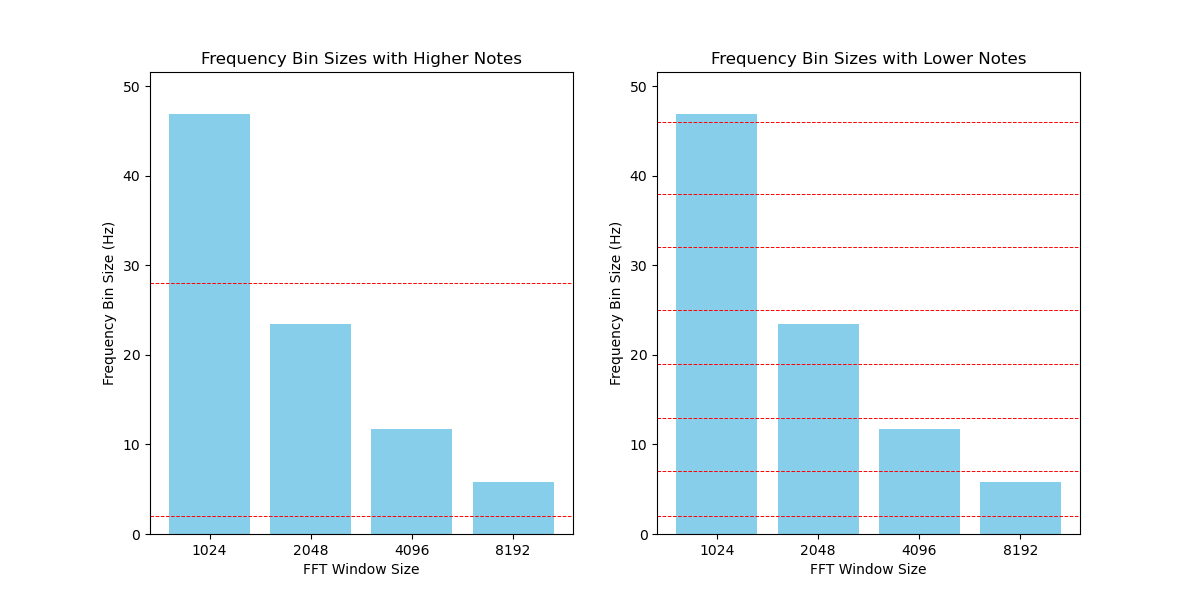
\includegraphics[width=\textwidth]{./images/fft_bin_size_chart.png}
    \caption{As the FFT window shrinks, different notes may fall into the same bin. Bars represent the bin sizes for various window sizes at 48kHz sampling rate and dashed lines show semitone intervals (the exact note values are irrelevant). For notes in the 4th octave, the window size can be smaller, but in the 2nd octave even 8192 samples is not enough to discern all pairs of semitones.\label{fig:fftBinSizeChart}}
\end{figure}

The difference between F2 and F\#2 is 5Hz which is smaller than the frequency bin of 8192 samples at 48kHz. They do not necessarily fall into the same bin but for the sake of correctness, it would be better to compute the FFT with a 16384 window size. This halves the frequency bin size and definitely accomodates differences even an octave lower. This introduces a significant amount of increased computation and is quite unnecessary as base singers do not realistically go this low. If the FFT implementation allows (many implementations require a power of 2), the window size should lie somewhere between 8192 and 16384 to lessen computations. For a 4Hz bin, $48000/x = 4 <=> x = 48000/4 = 12000$ 12000 samples would be enough to discern the lowest notes. 
% Narrowing the problem
\subsection{Real-time pitch detection}
One challenge with real-time pitch detection that emerged from the problem with the size of frequency bins was that for detecting lower base notes, the window size needed to be around 12000. However collecting 12000 samples at 48kHz takes 0.25s, which arguably is not real-time anymore. 
% Hypothesis, would need source or experimentation
As the bin size is the ratio of the sampling rate to the number of sample, one possible work around is to lessen the sampling rate when analyzing a base singer. If the sampling rate is cut to 12kHz, the latency (excluding the to compute the FFT) is cut down to 0.065s or 65ms. This approaches what might one argue to be real-time. \todo{There is a Bürck et all 1935 that states it takes 20-60ms but I can't find the article to verify it}. 
\subsubsection{Nyquist-Shannon sampling theorem}
The Nyquist-Shannon sampling theorem states that a signal needs to be sampled at 2 the rate of the highest frequency component. For instance the typical digital audio sampling rate is 44.1kHz to 48kHz, which is around 2x the highest frequency humans can hear. If, for the sake or argument, a base singer does not need to sing higher than 400Hz (around a G4), then the sampling rate can be reduced as low as 800Hz. Per the formula, $800/4 = 200$, the FFT can run on as small of a window as 200 samples (or 256 if it requires a power of 2).